\documentclass[12pt]{article}
\usepackage[margin=1in]{geometry}
\usepackage{setspace}
\usepackage{natbib}
\bibliographystyle{plainnat}
\usepackage{parskip}     % removes indent + adds vertical space
\setlength{\parindent}{0pt}   % just in case
\setlength{\parskip}{6pt}     % space between paragraphs

% --- Math + theorem environments + tables ---
\usepackage{amsmath,amssymb,amsfonts}
\usepackage{amsthm}
\usepackage{booktabs}
\usepackage{graphicx}
\graphicspath{ {figures/} }

% Shortcuts
\newcommand{\E}{\mathbb{E}}
\newcommand{\R}{\mathbb{R}}

% Load tcolorbox with theorem library
\usepackage[most]{tcolorbox}
\tcbuselibrary{theorems}

% Simple box for important stuff
\newtcolorbox{statementbox}[1]{%
    colback=white,
    colframe=black!70,
    coltitle=black,
    fonttitle=\bfseries,
    title={#1},
    enhanced,
    breakable,
    attach boxed title to top left,
    boxed title style={colback=gray!10}
}

% ---- TOCs ----
\usepackage{etoc}                 % flexible local tables of contents
\setcounter{tocdepth}{2}          % show up to subsections in the main ToC

% ---- Historical axiom box (title text black; date goes in title) ----
\usepackage[most]{tcolorbox}
\newtcolorbox{histaxiom}[1][]{%
  title={#1},                     % you write: Title — YYYY-MM-DD
  colback=gray!1,
  colframe=gray!60,
  coltitle=black,                 % ensure black title text
  borderline west={2pt}{0pt}{gray!70},
  enhanced,
  breakable,
  attach boxed title to top left,
  boxed title style={colback=gray!15}
}

% --- Helper to reduce boilerplate ---
% \HistAxiomEntry{Version title}{Status}{Date}{Old statement}{Issue}{Solution}
\newcommand{\HistAxiomEntry}[6]{%
  \begin{histaxiom}[#1]
    \textbf{Status:} #2\par
    \textbf{Date:} #3\par\medskip
    \textbf{Old statement.}\par #4\par\medskip
    \textbf{Issue.}\par #5\par\medskip
    \textbf{Solution.}\par #6
  \end{histaxiom}%
}

% --- Links ---
\usepackage{hyperref}

% --- For compact lists in notes ---
\usepackage{enumitem}

\title{Axiomatizing AI: Emergence Under Scaling}
\author{Isidor Manning}
\date{August 2025 - TBD}

\begin{document}
\maketitle
\tableofcontents
\newpage

\section{Introduction}
Emergent abilities in large language models (LLMs) are capabilities that appear suddenly and unexpectedly as the model scales up in size, data, and computational resources. When LLMs reach a certain size and complexity, they suddenly show capabilities that weren't seen before.

These abilities are not linearly predictable based on the model's performance on smaller scales, making them seem like qualitative leaps in capability rather than simple quantitative improvements. 

I am trying to create a mathematical theory of emergent capabilities in learning systems. These are the mysterious abilities—like arithmetic, reasoning, code generation—that seem to “just appear” when models are scaled up.

I’m beginning with emergent capabilities under scaling because it sits at the heart of the LLM revolution.

The recent breakthroughs in AI were powered by their emergent structures. They weren’t explicitly trained. They surfaced, and we don’t understand why.

GPT-2 wasn’t special. GPT-3 was. GPT-4 has reasoning capabilities that earlier models didn’t. These weren’t programmed. They emerged, and this gave birth to the AI The Big AI Boom. We don’t understand why. But scaling does something.

That’s the mystery I’m tackling.

\subsection{Questions}

\begin{itemize}
    \item Can I define a small set of general, falsifiable axioms that explain \textit{when and why} new capabilities emerge as we scale model resources?

    \item Can I propose a minimal set of mathematical assumptions such that from them, I can \textit{prove the existence} of critical thresholds—points at which certain capabilities emerge—and derive \textit{scaling laws} that match empirical observations?
\end{itemize}


\subsection{What This Involves—The Structure of My Work}
\begin{enumerate}
    \item \textbf{Defining the domain clearly:} \begin{itemize}
        \item What is a learning system?
        \item What are its resources? (tokens, parameters, compute)
        \item What is a capability, and how do we measure it?
    \end{itemize}

    \item \textbf{Proposing axioms:} \begin{itemize}
        \item They should be falsifiable—they might break under experiment which is an opportunity to refine them.
        \item They should be general—ideally true across many learning systems.
        \item They should be minimal—remove one, and the predictions break.
    \end{itemize}

    \item \textbf{Making predictions:} \begin{itemize}
        \item Derive theorems from the axioms.
        \item Predict phenomena like sharp transitions, power laws, universal curves.
        \item Run toy experiments (like modular addition or in-context learning) to test them.
    \end{itemize}

    \item \textbf{Refining the theory:} \begin{itemize}
        \item If the predictions break, I’ll revisit my definitions and axioms.
        \item I’ll aim to find deeper invariants, or maybe redefine what a “capability” even is.
        \item The process loops: definition → axiom → prediction → test → refinement.
    \end{itemize}
\end{enumerate}

\subsection{Why This Matters}
This isn’t just about LLMs or transformers. If successful, this theory could:

´\begin{itemize}
    \item Give us universal scaling laws for intelligence
    \item Predict when a new model will suddenly gain a powerful new ability
    \item Serve as the mathematical backbone of AI system design
    \item Possibly generalize to non-neural learning systems (e.g., biological, hybrid systems)
    \item Lay groundwork for a future theory of computational cognition
\end{itemize}

\section{The Domain of Emergence Theory}

We first need to clearly state the domain of our theory and answer questions like:

\begin{itemize}
    \item What are the objects of our theory?
    \item What are the resources being scaled?
    \item How do we measure the “emergent capability
    \item What is the scope of the theory?
\end{itemize}

The most important definition is the one about the learning systems. To be able to rigorously study emergent structures, we need to step away from the experimental notions of neural networks, Transformer architectures, etc., Instead, we need to find a mathematical abstraction at the perfect balance between usability and generality.

\subsection{Learning Systems And Recipes--What We Are Modeling}

My goal is to understand and model a system that learns and becomes more and more intelligent as it gets scaled up. More formally, I want to mathematically model a Transformer that gets trained and with emergent abilities surfacing as resources like compute, number of parameters, and training tokens increases beyond a certain threshold. 

We will denote this learning system by $S$.

We will also define a recipe, denoted by the Greek letter, $\Xi$, which will include information about the way we construct these intelligent models.

The following is a specific case of a learning system. In the next section we will see the general definition of a learning system.

\begin{statementbox}{Example: Learning System}

Let $S$ denote the specific learning system and $\Xi$ the recipe, given by

\[
S :=  (D,\mathcal L,A,\rho,\iota,F),\quad \Xi:= (\mathcal L,A,\rho,\iota,F)
\]

where:

\begin{itemize}
    \item $D\in \mathcal D$ is a subset of probability measures $\mathcal D$, and represents the data-generating process (training distribution and sampling scheme),

    \item $\mathcal L$ is the per-example loss (e.g., cross-entropy),
    \item $A$ is the training algorithm incl. schedule (optimizer family + LR/BS schedules),
    \item $\rho$ is regularization (weight decay, dropout, augmentations),
    \item $\iota$ is the initialization distribution,
    \item $F$ is the model architecture family.
    
\end{itemize}

\end{statementbox}

When we later say that “a capability emerges in $S$” we must be referring to a particular class of systems—a particular class of $S$. It is only then we can ask questions like “how does this behavior generalize over multiple $S$?” which will be a very important wonders to explore.

I will now begin generalizing this notion of a learning system and show how we will define $S$ as a point in a certain topological space.

\subsubsection{Topologizing The Learning System}
Now, the problem with a specific definition of $S$ (like the one provided above) is that it is not generalizable; deep learning systems vary a lot and much of the field is experimental so naturally this specific $S$ would just be a tiny fraction of possible models. This is the motivation for defining a more abstract and general framework for mathematically reasoning about AI models.  

\begin{statementbox}{Definition: Recipe}

The \textit{space of recipes} is a topological space $(\mathcal X , \tau_{\mathcal X})$ with underlying set $\mathcal X$ and topology $\tau _\mathcal X$.

Then, a \textit{recipe} is simply a point in the topological space $\Xi\in \mathcal X$.

\end{statementbox}

Intuitively, all we are saying is that the different ways we might create our end-model all live in the same topological space $\mathcal X$. 

Moreover, in the case of modern deep learning, a recipe $\Xi$ is usually itself a longer tuple with each component equipped with its own natural topology, making $\mathcal X$ into a topological product space. 

We do the same with the learning system:

\begin{statementbox}{Definition: Learning System}

Let $(\mathcal D, \tau_D)$ be a topological space of data-generating processes and $(\mathcal X, \tau_\mathcal X)$ a recipe space.

We define the \textit{space of learning systems} as the product topological space

\[
\mathcal S=(S,\tau_\mathcal S)=(\mathcal D , \tau_D)\times (\mathcal X, \tau_\mathcal X).
\]

Then, a \textit{learning system} is a point $S=(D,\Xi)\in \mathcal S$.

\end{statementbox}

Lastly, as you might have already thought, this definition of a learning system is indeed an axiom. I assume that everything we put into the recipe can form its topological space. We will state this axiom more formally once we get there.

However, by imposing this axiom, we can apply the theory of topology to our learning systems. With topology, we can make the idea of “two systems are similar” precise via neighborhoods and metrics. This will come in handy later on in our axioms. Topology could give us the formal language for talking about sequences of models, limits, continuity, convergence, and so on. When we later define what we mean by a “capability” we can also use topology to look at threshold sets and boundaries of emergence.

Before we move on, I will dedicate the next section to exemplify this abstraction. I will take our specific learning system we defined earlier, and define the topologies for each each space. This will get a bit theoretical but will hopefully strengthen the validity of this axiom.

\subsection{Example of a Learning System—The Canonical Learning Space Topology}

Going back to our old example where $\Xi=(\mathcal L, A, \rho, \iota, F)$, I will now propose some natural topologies for their respective topological space. In this example:

\begin{itemize}
    \item $(\mathcal L, \tau_{\mathcal L})$: per-example loss space,
    \item $(A, \tau_A)$: training algorithms,
    \item $(\rho, \tau_\rho)$: regularization schemes,
    \item $(\iota, \tau_\iota)$: initialization distributions,
    \item $(F, \tau_F)$: architecture families,
\end{itemize}
so:
\[
\mathcal S = (\mathcal D, \tau_D)\times (\mathcal L, \tau_{\mathcal L}) \times (A,\tau_A) \times (\rho,\tau_\rho) \times (\iota,\tau_\iota) \times (F,\tau_F).
\]

\subsubsection{Data-generating process $(\mathcal D, \tau_D)$}

Suppose $(X,d)$ is a metric space (e.g. sequences, tokens, or $\mathbb R^n$). Let $\mathcal P(X)$ denote the set of Borel probability measures on $X$. To treat data-generating processes as mathematical objects, we must equip $\mathcal P(X)$ with a topology, i.e. a notion of convergence of distributions.

\textbf{Topology $\tau_D$:} There are several possible notions of convergence for measures. In our setting, the natural choice is the **weak topology** $\tau_D$, under which a sequence $(D_n)$converges to $D$ if and only if

\[
D_n \Rightarrow D 
 \iff 
\int f  dD_n \longrightarrow \int f  dD
\quad \text{for all } f \in C_b(X),
\]

where $C_b(X)$ denotes the space of bounded continuous functions on $X$.

This topology is standard in probability theory and stats. It expresses the idea that probability measures are close whenever they yield similar expectations for all continuous observables. In particular, weak convergence formalizes the intuition that empirical distributions converge to the true data distribution as sample size grows.

\subsubsection{Loss functions $(\mathcal L, \tau_\mathcal L)$}

$\mathcal L$ is the set of per-example losses, which we treat as measurable functions $\ell: Y \times \hat{Y} \to \mathbb R_{\geq 0}$.

\textbf{Topology $\tau_\mathcal L$:} Uniform convergence on compact sets, or the $L^p$-topology with respect to the data distribution $D$.

Losses are functionals. Their behavior is stable if they converge uniformly. This makes the risk functional $\mathbb E_D[\ell]$ continuous.

\subsubsection{Training algorithms $(A, \tau_A)$}

$A$ is the set of algorithms mapping data with parameters and output updated parameters.

We can think of each algorithm as a map $T: \Theta \times \mathcal D \to \Theta$, where $\Theta$ is the parameter space.

\textbf{Topology $\tau_A$:} compact-open topology (standard for function spaces), or equivalently pointwise convergence on compacts.

It ensures “if two optimizers are close, then their parameter updates are close on compact sets of inputs.”

\subsubsection{Regularization $(\rho, \tau_\rho)$}

$\rho$ are maps or functionals modifying training dynamics (e.g. penalties, dropout distributions, augmentations).

These are again functions/transformations.

\textbf{Topology $\tau_\rho$:} operator norm topology if regularization is linear, or compact-open topology if nonlinear.

It ensures stability under small changes in the regularization scheme.

\subsubsection{Initialization distributions $(\iota, \tau_\iota)$}

$\iota$ is a probability measure on the parameter space $\Theta$.

\textbf{Topology $\tau_\iota$:} weak topology on probability measures (same as for data $D$).

Initialization schemes are compared by the limiting distribution of parameter samples.

\subsubsection{Architecture families $(F, \tau_F)$}

$F$ is the set of model architectures, thought of as families of functions $f_\theta:  X \to Y$parameterized by $\theta \in \Theta$.

\textbf{Topology $\tau_F$:} Pointwise convergence of functions ($f_n \to f$ if $f_n(x)\to f(x)$ for all $x$). Or, stronger, uniform convergence on compact subsets of $X$.

Architectures are function classes; topologies of function spaces are standard here. Uniform-on-compacts is natural for deep learning since inputs are usually bounded sequences.

\subsection{The Recipe-Local Neighborhood}

To say speak of ”nearness” between learning systems’ recipes, later on in our axioms we need to define a certain “Learning Space Neighborhood” This is what we will do now.

\subsubsection{The Data Distance}

To clearly define this neighborhood, we will need a couple of metrics, starting off with the data distance.

\begin{statementbox}{Definition: The Data Distance}

Let $(\mathcal Z,d_\mathcal Z)$ be a Polish sample space (i.e., a topological space that is separable and completely metrizable). Fix $p\ge 1$ and define

\[
\mathcal D := \mathcal P_P(\mathcal Z)\\=\left\{
D:\text{Borel probability on }\mathcal Z \text{ with } \int d_\mathcal Z (z,z_0)^pD(dz)<\infty
\right\}
\]

Equip $\mathcal D$ with the Wasserstein metric $W_p$. This induces the topology $\tau_D$. Then, our \textit{data distance} as

\[
d_D(D,D'):= W_p(D,D')
\]

where $D,D'\in \mathcal D$

\end{statementbox}

\subsubsection{The Recipe Distance}

Next, we move on to the recipe distance, which, as it sounds, will help measuring the “distance” between different recipes in $(\mathcal X, \tau_\mathcal X)$.

First, we need to split categorical vs. continuous parts of $\phi_\Xi$. Here are a few examples of what I mean with “categorical features” and “continues features”:

\begin{itemize}
    \item \textbf{Categorical features $c(\Xi)$} (one-hot or simple labels): \begin{itemize}
        \item optimizer family (AdamW, SGD, Lion, …)
        \item schedule shape (cosine, linear, step, …)
        \item architecture family (attn-only, full transformer, conv-mixer, …)
        \item positional encoding type (sinusoidal, RoPE, ALiBi, …)
        \item normalization / activation (LayerNorm vs. RMSNorm; ReLU/GELU/SiLU)
        \item precision regime (bf16, fp8, 8-bit optimizers)
    \end{itemize}
    \item \textbf{Continuous features $h(\Xi)$} (we use logs for positive scales): \begin{itemize}
        \item $\log$ weight decay, dropout rate, label smoothing
        \item $\log $ init variance or fan-in scale
        \item optimizer hyperparams ($\beta_1$, $\beta_2$, $\epsilon$, $\alpha$), gradient clip
        \item schedule shape parameters (e.g., warmup fraction), not LR magnitude if you allow ±10% jitter
    \end{itemize}
\end{itemize}

\begin{statementbox}{Definition: The Recipe Distance}

Let $C$ be the set of categorical features. Give $C$ the discrete topology. 

Secondly, let $h:\Xi \to \mathbb R^p$ be the vector of continuous hyperparameters in log-coordinates. Give $\mathbb R^p$ the Euclidian topology. Then, define $\phi:\Xi \to C\times \mathbb R^p$ by

\[
\phi(\Xi)=(c(\Xi),h(\Xi))
\]

Define $\tau_\Xi$ to be the initial topology making $\phi$ continuous when $C\times \mathbb R^p$ has the product topology (discrete $\times $ Euclidian). Concretely, a basic neighborhood of $\Xi$ is

\[
\{\,\Xi':\ c(\Xi')=c(\Xi)\ \text{and}\ \|W(h(\Xi')-h(\Xi))\|_2<\varepsilon_\Xi\,\},
\]

for some diagonal

\[
W=\text{diag}\!\left( \frac 1 {\tau_1} , \dots , \frac 1 {\tau_p}\right)\quad \text{and}\quad \epsilon_\Xi >0.
\]

The \textit{recipe distance} is defined as

\[
d_\Xi(\Xi,\Xi') :=
\begin{cases}
\|W(h(\Xi)-h(\Xi'))\|_2, \text{ and } c(\Xi)=c(\Xi')\\
\infty, \text{ and } c(\Xi)\neq c(\Xi')
\end{cases}
\]

where $d_\Xi(\Xi,\Xi')\in [0,\infty]$.

\end{statementbox}

This is an extended metric. Its open balls are exactly the sets above and they generate $\tau_\mathcal X$. Note that the choice of positive tolerances $\tau_j$ (i.e., diagonal $W$) does not change the topology. Also, log coordinates require positive parameters; if some hyperparameter can be zero, we might want to use $\log(\alpha+\cdot )$ with some tiny $\alpha>0$.

Choose per-dimension tolerances $\tau_j>0$ that encode “how much change counts as small”

\[
d_{\text{cont}}(\Xi,\Xi') 
:= \left\| W\,\big(h(\Xi)-h(\Xi')\big)\right\|_2,
\quad W:=\mathrm{diag}\!\left(\frac{1}{\tau_1},\dots,\frac{1}{\tau_p}\right)
\]

So a change equal to one tolerance contributes $1$ along that coordinate. Now we can combine the two into one recipe distance,

\[
d_\Xi(\Xi,\Xi') :=
\begin{cases}
d_{\text{cont}}(\Xi,\Xi'),& \text{if } c(\Xi)=c(\Xi')\\
\infty, &\text{otherwise}
\end{cases}
\]

\subsubsection{The Learning System Neighborhood}

\begin{statementbox}{Definition: The Learning System (LS) Neighborhood}

With the recipe and data distances defined, the LS neighborhood is exactly the basic open set:

\[
\mathcal U(S)=\Bigl\{S'=(D',\Xi'):d_D(D,D')\le\varepsilon_D, d_\Xi(\Xi,\Xi')\le\varepsilon_\Xi\Bigr\}
\\= B_{W_p}(D,\varepsilon_D)\times B_{d_\Xi}(\Xi,\varepsilon_\Xi)
\]

So $\{\mathcal U (S;\epsilon_D,\epsilon_\Xi)\}$ is a neighborhood basis at $S$ in $\mathcal S$. 

\end{statementbox}

\subsubsection{Studying Learning Systems}

With this $S$ we could you define equivalence classes of systems where different choices yield the same scaling laws. For example, two different systems, $S$ and $S'$, might belong to the same universality class for emergence under a specific capability.

\subsection{Resources And The Feature Map}

Linear algebra is arguably the core of LLMs. Thus, it makes sense for us to start exploring the treating of abstract concepts like ”resources,” as abstract vectors. We want to define this in the first place because it will allow us to theoretically understand how resources affect the learning system. In other words, this defines the independent variables that control our learning system $S$.

\begin{statementbox}{Example: Resources}

Let resources be a positive vector $R\in \mathbb R^d_{>0}$ with a feature map $\psi:\mathbb R^d_{>0}\to \mathbb R^d$, defined by

\[
\psi(R):=(\log R_1,\dots,\log R_d)\in \mathbb R^d
\]

For example, we might have $R=(N,P,T)$, where:
\begin{itemize}
    \item $N$ is the number of training tokens/examples,
    \item $P$ is the number of parameters from $F$,
    \item $T$ is the optimization budget (number of optimization steps or total FLOPs).
\end{itemize}

\end{statementbox}

\subsubsection{Topologizing the Resource Vector--The Resource Space}

\begin{statementbox}{Definition: Resources}
    We define the \textit{resource space} as $\mathcal R=(\R^d_{>0}, \tau_{\R^d_{>0}})$ the set of positive vectors of dimension $d$ with standard Euclidean topology $\tau_{\R^d_{>0}}$.

    When a feature map $\psi:\mathcal R \to \R^k$ is used, we take the pullback topology induced by $\psi$.
\end{statementbox}

This allows us to speak of neighborhoods of resource configurations, interior points of superlevel sets, and continuity of the capability map. 

\subsection{The Training Map}

Training deep models is inherently stochastic: shuffling data, random initialization, dropout, augmentation noise. To reason about outcomes rigorously, we need to model training not as a deterministic function but as a stochastic map from learning system + resources to trained states. Probability theory gives us the language to treat “random training outcomes” as distributions over parameters, rather than loose hand-waving.

\begin{statementbox}{Definition: The Training Kernel}

Define the stochastic training map as a Markov kernel

\[
K :\mathcal S \times \mathbb R^d_{>0} \longrightarrow B(\Theta)
\]

where for each system–resource pair $(S,R)$, the kernel $K(S,R)$ specifies a probability measure on the parameter space $\Theta$. Sampling $\theta\sim K(S,R)$ corresponds to training a model with system $S\in \mathcal S$ under resources $R\in \mathbb R^d_{>0}$, with all stochasticity folded into the randomness of $K$. Here:

\begin{itemize}
    \item $\Theta$ is the space of model states (like weight vectors of a neural net), typically equipped with the Borel Sigma-algebra from its ambient topological structure.
    \item $B(\Theta)$ is the space of Borel probability measures on $\Theta$. Each elements of $B(\Theta)$ represents a distribution over trained states.
    \item $K$ is a measurable assignment of probability distributions: for fixed $(S,R)$, $K(S,R)$ is a probability measure on $\Theta$; for measurable sets $B \subseteq \Theta$, the map $(S,R)\mapsto K(S,R)(B)$ is measurable.
\end{itemize}

\end{statementbox}

Equivalently, the kernel may be realized via a measurable map

\[
\text{Train}:\mathcal S \times \mathbb R^d_{>0} \times \Omega\longrightarrow \Theta
\]

defined on an underlying probability space $(\Omega, \mathbb P)$ of randomness sources such that

\[
K(S,R)=\mathbb P \circ \text{Train}(S,R,\omega)^{-1}
\]

where:
\begin{itemize}
    \item $(\Omega,\mathbb P)$ is an abstract probability space encoding all sources of randomness in training (seeds, noise, etc.).
    \item $\text{Train}$ is the measurable training function that takes a system, a resource, and a randomness seed $\omega\in \Omega$ to a concrete trained state $\theta\in \Theta$.
    \item $\mathbb P \circ \text{Train }(S,R,\omega)^{-1}$ is the induced distribution on parameters $\theta$ when randomness $\omega$ is sampled from $\mathbb P$.
\end{itemize}

Think of the training map as a dice roll conditioned on system $S$ and resources $R$. Sometimes you get a “good seed,” sometimes a bad one—but what matters mathematically is the distribution of possible trained states. By formalizing this randomness, we can later ask: do emergent capabilities appear consistently, or only under rare lucky seeds? This connects to our earlier definitions by making the learning system $S$ and resources $R$ the inputs of a stochastic process.

Training outcomes are never deterministic: even fixing system design and resource budget, two training runs may lead to different states $\theta$. To model this rigorously, we treat training as a Markov kernel, i.e. a map from inputs $(S,R)$ to probability distributions on outcomes. This allows us to:

\begin{enumerate}
    \item Average over randomness when defining expected capability,
    \item Distinguish structural emergence from “lucky seeds,” and
    \item Align with probability theory, where kernels are the natural object for stochastic transformations.
\end{enumerate}

Thus, this construction makes explicit what practitioners know implicitly: training defines not one point, but a distribution of possible models.

\subsection{The Predictor Map}

The training kernel $K(S,R)$ tells us \textit{where you land in weight space.} But we also need to define a predictor, $\Pi_\theta$, that tells us \textit{what those weights predict.} Many results (calibration, ensembling, metric design) live entirely on the inference side and shouldn’t be conflated with training randomness.

\begin{statementbox}{Definition: The Predictor Map}

Let $(X,Y)$ be the input/output spaces. Define $\mathcal P (Y)$ as the set of probability measures on $Y$. A trained state $\theta$ induces a stochastic kernel, called the predictor map,

\[
\Pi_\theta:X\to \mathcal P(Y),\quad x\mapsto \Pi_\theta(\cdot \mid x),
\]

i.e., for each input $x$, $\Pi_\theta(\cdot \mid x)$ is a probability distribution on outputs $Y$—the model’s belief over outputs for input $x$.

\end{statementbox}

The reason we keep both is because they answer different questions: How do we sample trained models? ($K$) vs. What does a specific trained model believe about outputs? ($\Pi$). Keeping them separate gives us exact, composable statements and avoids silent changes in $m_\Phi$ when averaging across seeds or checkpoints.

\subsection{The Composition of $\Pi_\theta$ and $K$}

For completeness, we can define a “mixture predictor,”

\[
\bar \Pi _{S,R}(\cdot \mid x):= \int _\Theta \Pi_\theta(\cdot \mid x)dK(S,R)(\theta).
\]

\subsection{What $\Pi_\theta$ looks like in common cases}

\subsubsection{Classification (finite labels)}
\[
\mathcal Y=\{1,\dots,K\} . \\
\Pi_\theta(\cdot\mid x)=\mathrm{softmax}(z_\theta(x))\in\Delta^{K-1}
\]

Examples of $\mathcal U_\Phi$:
\begin{itemize}
    \item probability of the correct label $\Pi_\theta(\{y\}\mid x)$ (bounded, continuous),
    \item clipped/normalized log-prob, or the Brier score mapped to $[0,1]$.
\end{itemize}

\subsubsection{Regression (real-valued)}

\[
\mathcal Y=\mathbb R
\]

Choose a predictive family, e.g. Gaussian

\[
\Pi_\theta(\cdot\mid x)=\mathcal N(\mu_\theta(x),\sigma^2_\theta(x)).
\]

Examples of $\mathcal U_\Phi$:
\begin{itemize}
    \item mass in a tolerance band $\Pi_\theta([y-\varepsilon,y+\varepsilon]\mid x)$ (proper for the induced set-loss, bounded),
    \item a normalized CRPS/log-likelihood mapped into $[0,1]$ (keep it bounded and continuous).
\end{itemize}

\subsubsection{Seq2seq Modeling}

\[
\mathcal Y=\mathcal V^{*} \quad \text{(finite strings)}
\]

$\Pi_\theta(\cdot\mid x)$ is the autoregressive distribution $\prod_t p_\theta(y_t\mid x,y_{<t})$.

Examples of $\mathcal U_\Phi$:
\begin{itemize}
    \item per-token geometric mean probability
    \[
    \exp\!\left(\frac{1}{|y|}\log \Pi_\theta(y\mid x)\right)\in(0,1],
    \]
    \item probability mass of the acceptable set $A(x)$ (if multiple outputs are valid): $\Pi_\theta(A(x)\mid x)$ or its log mapped to $[0,1]$.
\end{itemize}

\subsection{Quantifying Emergence}

\subsubsection{Capability}

Emergence is only meaningful relative to a capability: we need to specify “what task” the system should perform and “how” we measure success. Mathematics forces us to be precise: a capability is not just “the model can translate,” but a tuple of input/output spaces, evaluation distribution, and a scoring rule. This makes capabilities comparable across learning systems.

\begin{statementbox}{Definition: Learning Task}

Let $\mathcal T _\Phi=(X,Y,g_\Phi, p_\Phi)$ be the \textit{task} with input/output spaces $(X,Y)$, ground truth $g_\Phi(x,y)$, and evaluation distribution $p_\Phi(x,y)$. 

\end{statementbox}

\begin{statementbox}{Definition: Learning Utility}

Let $\mathcal U_\Phi : \mathcal P \times Y \to[0,1]$ be the \textit{utility}-—a bounded and continuous scoring rule mapping predictions to $[0,1]$ (e.g., probability on the true label, normalized log score).

\end{statementbox}

\begin{statementbox}{Definition: Capability}

A \textit{capability} is a pair $\Phi:=(\mathcal T_\Phi, \mathcal U _\Phi)$.

\end{statementbox}

A capability here is an experimental setup: what data we feed, what counts as correct, and how we score performance. Framing it rigorously means we can talk about emergence as “a sharp change in expected capability under scaling,” not just “it feels like the model suddenly gets good at X.”

\subsubsection{State Score}

Given a trained state $\theta$ (which we get from $\Pi_\theta$), we need a well-defined numerical quantity that says how good that state is at a capability. This is where the state-level score $M_\Phi(\theta):\mathcal S \times \mathcal R \to [0,1]$ comes in: it evaluates one fixed trained model against the capability’s scoring rule. We restrict to bounded, continuous scoring rules to ensure mathematical tractability (continuity guarantees smooth dependence on model parameters).

\begin{statementbox}{Definition: State-Level Score}

For a trained state $\theta$, we define the \textit{state-level score}, $M_\Phi$, as 

\[
M_\Phi(\theta)=\mathbb E_{(x,y)\sim p_\Phi}\Big[\mathcal U_\Phi\big(\Pi_\theta(x),y\big)\Big]
\]

where:
\begin{itemize}
    \item $\Pi_\theta$ is the model’s predictive object at parameter state $\theta$: a mapping from inputs to probability distributions over outputs.
    \item $\mathcal U_\Phi$ is a scoring rule that knows how to take that predictive object and the ground-truth $y$ and return a number in $[0,1]$.
    \item $M_\Phi(\theta)$ is continuous in $\theta$ if $\Pi$ and $\mathcal U _\Phi$ are continuous and dominated convergence applies.
\end{itemize}

\end{statementbox}

So we feed $\Pi_\theta(\cdot\mid x)$ and $y$ into $\mathcal U_\Phi$ (probability of acceptable set, normalized log prob, Brier-like score, etc.), then average over the eval distribution $p_\Phi$.

A state score is just “how well this particular trained model did on the task.” It’s the bridge between a single point in parameter space and the notion of capability. This plugs back into our topological view: since the parameter space $\Theta$ is topologized, continuity ensures that small perturbations of parameters lead to small changes in performance.

\subsubsection{Expected Capability}

Because training is stochastic, one state score is not enough: we care about average behavior across seeds and sources of randomness. The expected capability $m_\Phi(S,R):\mathcal S \times \mathcal R \to [0,1]$ aggregates over randomness, producing a stable number that depends only on the system $S$ and resource vector $R$. This expectation is crucial. Otherwise, emergence could appear or disappear based purely on unlucky runs.

\begin{statementbox}{Definition: Seed-Averaged Capability}

For a trained state $\theta$, we define the \textit{seed-averaged} capability, $m_\Phi$, as

\[
m_\Phi(S,R)=\mathbb E_{K_{S,R}}\!\big[M_\Phi(\theta)\big]
=\int_\Theta M_\Phi(\theta)\,K_{S,R}(d\theta)
\]

\end{statementbox}

The expected capability is the true curve we want when we plot performance vs. scale: the seed-averaged trajectory of learning. It’s the counterpart of Shannon’s expected information measure — stripping away incidental noise to reveal the systematic structure. This is where all definitions unify: $S$, $R$  (resources), training randomness, and capability definitions come together in a single function $m_\Phi(S,R)$. Emergence then becomes a property of this function’s shape.

\subsection{Representability}

Not all learning systems can have certain abilities emerge. I cannot train an MLP with 2 layer, expecting to achieve a $m_\Phi>0.99$ on a parity capability with length 64. That's not how machine learning works, so naturally we will need tools to answer the question "when is a capability $\Phi$ representable by a learning system $S\in \mathcal S $?"

\begin{statementbox}{Definition: Representability of Capability}
    Let $\tau \in (0,1)$ be a performance threshold (e.g., $\tau=0.90$). Define the \textit{superlevel set} as
    \[
        E_\tau =\{ S\times R \in \mathcal S \times \mathcal R: m_\phi(S,R)>\tau \}.
    \]
    Then, we say $\Phi$ \textit{is representable} by the learning system $S$ at level $\tau$, if and only if $E_\tau$ is nonempty and has nonempty interior in $\mathcal S \times \mathcal R$.
\end{statementbox}

Empirically, we replace $m_\Phi$ by its seed-averaged estimate and require a lower confidence bound to exceed $\tau + \epsilon$ on a neighborhood, ensuring robustness to stochasticity.

Using "$>\tau$" makes $E_\tau$ open whenever $m_\Phi$ is continuous, so "hard interior" means "there's a neighborhood of configurations where the capability holds," not a single lucky point.

\begin{statementbox}{Definition: Representability threshold along a resource axis}
    Fix a coordinate $R_i\in \mathcal R$, holding both $\Xi$ and $R_j$, $i\ne j$ constant. Then define
    \[
        R_\Phi = \inf \{ R_i : m_\Phi (\Xi, R_i\times R_j)>\tau\}
    \]
    If this infimum is finite and the set $\{ R_i : m_\phi >\tau\}$ contains an open interval above it, we say "$\Phi$ \textit{emerges along} $P$ \textit{at} $R_\Phi$" for that slice.
\end{statementbox}

At last, we have a function, $m_\Phi$ that reflects performance on a capability $\Phi$. We now want to come up with a set of axioms for this function and the definitions around it that reflects the emergence of tasks we see in empirical results. Here’s the mental picture you can keep in your mind:

\[
(S,R)\ \xrightarrow{\ K\ }\ \theta\ \xrightarrow{\ \Pi\ }\ \Pi_\theta(\cdot\mid x)\ \xrightarrow{\ \mathcal U_\Phi\ }\ \text{score}\in [0,1]\ \xrightarrow{\ \mathbb E_{x,y},\ \mathbb E_\theta\ }\ m_\Phi
\]

\subsection{Scope of the Theory}

The framework developed here aims to provide a mathematical language for describing capability emergence in large learning systems. To remain general yet precise, we delimit what phenomena are modeled and what lies beyond the present theory.

\subsubsection{In Scope}

\begin{itemize}
    \item \textbf{Learning systems} $S$ trained via stochastic optimization on large datasets, represented abstractly through data distributions and recipes.
    \item \textbf{Resource scaling $R \in \mathbb R^d_{>0}$:} we explicitly model the effect of increasing data, parameters, compute, or other resource coordinates.
    \item \textbf{Training stochasticity:} modeled at the level of distributions over trained states via the Markov kernel $K$.
    \item \textbf{Capabilities $\Phi$:} defined abstractly as tasks and evaluation utilities, with performance measured by state-level scores and seed-averaged expectations.
    \item \textbf{Emergence:} captured through the local and asymptotic behavior of capability measures$m_\Phi(S,R)$.
\end{itemize}

\subsubsection{Out of Scope For Now}

\begin{itemize}
    \item \textbf{Fine-grained optimization dynamics:} e.g. gradient noise, implicit bias of optimizers, trajectory-level analyses.
    \item \textbf{Data modality specifics:} text, vision, multimodal architectures, etc. are not distinguished; the data distribution $D$ is treated abstractly.
    \item \textbf{Human-in-the-loop effects:} reinforcement learning from human feedback, preference modeling, or interactive supervision.
    \item \textbf{Societal and alignment considerations:} while motivating, these lie outside the scope of the formal mathematics here.
\end{itemize}

\section{Axiomatizing Emergence}

\subsection{What Do We Want From Our Axioms?}

When creating and refining our axioms, we want them to do 3 things:

\begin{enumerate}
    \item \textbf{Predictive power:} from the axioms we can derive a \textit{representation theorem} that makes \textit{quantitative} predictions. In our case, the representation theorem are the scaling laws we see in LLMs.
    \item \textbf{Invariance:} claims don’t depend on irrelevant choices; our axioms shouldn’t depend on basis rotations, unit rescalings, and so on.
    \item \textbf{Smallest set:} nothing redundant; each axiom’s removal should break the key derivation to our representation theorem.
\end{enumerate}

We know that the scaling laws work. So what must a measure of capability, $\Phi$, satisfy under scaling? So what properties should capability emergence obey?

\subsection{Current Axioms}

\subsubsection{Axiom 1}

\begin{statementbox}{Axiom 1 (A1) - Monotone Capability}

For any representable capability $\Phi$ and learning system $S$, the expected capability $m_\Phi(S,R)$ is coordinate‑wise non‑decreasing in each resource $\{R^{(i)}\}$. 

Empirically, we accept $\epsilon$‑monotonicity at confidence $\alpha$: for every adjacent pair along a resource sweep,

\[
\text{LCB}_{1-\alpha}\left[m_\Phi\bigl(R_{i+1}\bigr) - m_\Phi\bigl(R_i\bigr)\right]\ge -\epsilon,
\]

where:
\begin{itemize}
    \item $\alpha$ is the one-sided error rate (e.g. $0.05$),
    \item $\text{LCB}_{1-\alpha}$ is the lower confidence bound (LCB) at confidence level $1-\alpha$,
    \item $\epsilon=\epsilon_\text{stat}+\epsilon_\text{num}$ is a pre-declared tolerance.
\end{itemize}

\end{statementbox}

\textbf{Intuitively,} more data/parameters/compute shouldn’t \textit{hurt} a capability in expectation. It rules out “perverse” regressions that are really optimization noise; it’s a weak, falsifiable regularity to build on. (Violations typically indicate under/over-training, metric noise, or a recipe bug.)

Without the precondition that $\Phi$ must be representable by $S$, we get flat noise around chance that appears to “violate” monotonicity.

When it comes to choosing the tolerances, $\epsilon_\text{stat}$ can be chosen from your uncertainty. One fast choice is:
\[
\epsilon_\text{stat} = c\cdot \max _ i \text{SE} _i,\quad c\in [1,2],
\]
where:
\begin{itemize}
    \item $\text{SE}_i $ is the standard error of $m_\Phi$ at setting $i$,
    \item $c$ reflects how conservative you want to be.
\end{itemize}

$\epsilon_\text{num}$ cover floating-point granularity (e.g. $5\times 10^{-7}$ for float32 contexts).

So given two adjacent resource settings $R_i,R_{i+1}$, we observe the seed-averaged capability difference:
\[
\Delta_i = m_\Phi(S,R_{i+1})-m_\Phi(S,R).
\]

Because training is stochastic, $\Delta_i$ has sampling uncertainty. Let $\widehat \Delta_i$ be the empirical mean across seeds, and let $\text{SE}(\widehat \Delta_i)$ be its standard error. The LCB at confidence level $1-\alpha$ is:
\[
\text{LCB}_{1-\alpha}(\Delta_i)=\widehat \Delta_i - z_{1-\alpha} \text{SE}(\widehat \Delta_i),
\]
where $z_{1-\alpha}$ is the quantile of the standard normal. If $\text{LCB}_{1-\alpha}(\Delta_i)>-\epsilon$, then with high confidence the true change is non-negative up to tolerance $\epsilon$. If it goes below $-\epsilon$, then we have evidence of a real monotonicity violation, not just numerical or sampling noise.

\subsubsection{Axiom 2}

\begin{statementbox}{Axiom 2 (A2) - Curve Fit Quality}

There exists a direction $\alpha\in \mathbb R^d$, an onset $s^*\in \mathbb R$, a width $w>0$, and a smooth increasing $f:\mathbb R\to [0,1]$ such that
    
\[
m_\Phi(S,R)\approx f(s'),\quad f\left ( \frac{\alpha^\top \psi (R)-s^*}{w}\right),
\]

where:

\begin{itemize}
    \item $s^*$ is the resource level at the midpoint of rise (e.g., $m_\Phi=0.5$ for logistic $f$),
    \item $w$ controls sharpness (smaller $w$ means sharper; for logistic $f$, slope at onset = $1/(4w)$ and the 10-90% rise $\approx 4.394w$),
    \item $s'$ is is dimensionless.
\end{itemize}

The quality of “$\approx$” is quantified by a collapse error

\[
\mathrm{CE}(\alpha, s_\star, w, f)
:=\sqrt{\frac{1}{\sum_i w_i}\sum_i w_i\big(m_{\Phi,i}-f(s'_i)\big)^2},\quad
w_i=\tfrac{1}{\widehat{\mathrm{Var}}[m_{\Phi}(S,R_i)]}  
\]

computed over runs $\{(S,R_i)\}_i$ with seed-averaged measurements $m_{\Phi, i}$. Define the optimized \textit{collapse error:}

\[
\mathrm{CE}^*:= \min_{\alpha, s^*,w,f\in \mathcal F_\uparrow} \mathrm{CE}(\alpha,s^*,w,f),
\]

where $\mathcal F_\uparrow$ is a class of monotone S-curves. $\mathrm {CE}^*$ must be reported on held-out runs.

\end{statementbox}


\textbf{Intuition:} All resource settings act as movement along one effective axis $s=\alpha^\top\psi(R)$. After centering by $s^*$ and scaling by $w$, every run lands on the same S-curve** $f$. The collapse error is “how far the cloud is from a 1-D curve” after the best possible projection.

\textbf{Why have it:} This turns “emergence under scaling” into a falsifiable claim with a single exchange-rate vector $\alpha$ and two interpretable scalars $(s^*,w)$. If the 1-D law is nearly as predictive as a flexible multi-knob surface—and better than any single resource alone—you’ve extracted a predictive primitive for \textit{when} (via $s^*$) and \textit{how sharply} (via $w$) a capability turns on, independent of the particular mix of resources.

\subsubsection{Axiom 3}

\begin{statementbox}{Axiom 3 (A3) - Finite-size scaling near transition}

Fix a learning system $S$ and a recipe-local neighborhood $\mathcal U(S)$; only seeds and small LR/BS jitters vary. Assume A2 holds with feature map $ \psi:\mathbb R^d_{>0}\!\to\mathbb R^d$. Then there exist $(\alpha, s_\star, w, f)$ for which A2 holds such that, for every $S'\in\mathcal U(S)$:

\begin{enumerate}[label=\roman*.]
    \item The projection direction $ \alpha$ (the trade-off between resource components in $\psi(R)$) is the same for nearby systems $S'$ in your recipe-local neighborhood:
    \[
    \cos\angle(\alpha,\alpha_{S'}) \ge 1-\varepsilon_\alpha,
    \]
    \item The location of the turn-on (midpoint of the S-curve in effective resource units) is consistent across $S'$:
    \[
    |s_\star - s^\star_{S'}| \le \varepsilon_{s},
    \]
    \item The sharpness of the transition is stable:
    \[
    |w - w_{S'}| \le \varepsilon_{w},
    \]
    \item After re-fitting, the collapse error isn’t worse than before by more than a small $\eta$:
    \[
    \frac{\mathrm{CE}^\star_{S'}}{\mathrm{CE}^\star_{S}} \le 1+\eta.
    \]
\end{enumerate}

and, near onset, the transition width obeys a multiplicative shrinkage law

\[
w(R)\approx C\exp\big(-\nu_\Phi^\top \psi(R)\big)
\quad\text{with}\quad \nu_\Phi\in\mathbb R^d_{\ge 0},\ C>0
\]

\end{statementbox}

\subsubsection{Axiom 4}

\begin{statementbox}{Axiom 4 (A4) - Invariance}

Conclusions about $\Phi$ must be invariant under linear reparameterizations of internal representations. Tests should rely on basis-invariant metrics (e.g., linear-probe accuracy, CKA/CKA-like, or SAE feature spaces), not neuron-level counts.

\end{statementbox}

\subsubsection{Axiom 5}

\begin{statementbox}{Axiom 5 (A5) - Topology}

\((\mathcal D, \tau_D)\) and \((\mathcal R, \tau_\mathcal R)\) are topological spaces. Their product \(\mathcal S = \mathcal D \times \mathcal R \) induces a predictor map,
\[
G:\mathcal S \to \{\Pi_\theta : X\to \mathcal P (Y)\}.
\]
For fixed $R$, $G$ is continuous in the function-space topology. 

\end{statementbox}

Continuity is assumed only for predictors, not for internal representations.

\textbf{Intuition:} This axiom does not describe \textit{what} a recipe or data-generating process is internally. It only asserts that they admit a topology, i.e. a notion of continuity and convergence. This restriction is deliberate: it ensures that we can study properties of learning systems (such as capabilities and emergence phenomena) using the language of topology.

\section{Experimentation—Trying My Absolute Best To Break My Theory}

When you axiomatize an empirical domain like modern AI, you’re not declaring truths, but instead you’re proposing tight, testable axioms that compress messy behavior into a few operational claims. Each axiom turns vague talk of “emergence” into specific predictions about a continuous order parameter that should rise along an effective resource axis, align across different ways of spending resources, stay stable within a defined training regime, and be immune to arbitrary reparameterization. Making these axioms falsifiable maximizes information gain. A confirming result means the lens has real predictive bite; a failure tells you exactly where the world refuses the simplification—which knob (data, parameters, steps, context length, precision, data quality) breaks curve collapse, which metric creates mirages, which recipe shift moves the onset or sharpness. In this hybrid program, experiments don’t just “validate” theory; they carve its domain of validity, turning broad conjectures into precise, recipe-local laws and revealing the minimal assumptions under which capability transitions actually behave like scaling phenomena worth proving later.

\subsection{Shared setup (for all experiments)}

\begin{itemize}
    \item Systems And recipes: keep a fixed recipe $\Xi$ (AdamW + cosine schedule, bf16, attention-only transformer, tied embeddings) and define your recipe-local neighborhood via your recipe distance with hard categoricals and tolerance-weighted Euclidean on continuous knobs (±10% LR/WD, ±0.02 dropout, etc.). This makes A3’s “locality” operational.
    \item Training map $K$ and predictor $\Pi_\theta$: compute 
    \[
    m_\Phi(S,R)=\mathbb E_{\theta\sim K(S,R)}[M_\Phi(\theta)]
    \]
    with continuous scoring $\mathcal U_\Phi$ (probability mass on the acceptance set or normalized log-prob), not thresholds (your A6-style precaution).
    \item \textbf{Resources:} start with $R=(N,P,T)$ and $\psi(R)=\log R$; later add a 4th coordinate (context length $L$, or quality $Q$).
    \item \textbf{Grid:} small, dense patches beat huge sweeps. Typical 18–36 runs per capability: $P\!\in\!\{0.5,1,2\}$M; $N\!\in\!\{1,2,4\}$M tokens; steps so tokens $\approx N$; 2 seeds each.
    \item \textbf{Models:} 1–4 layer attn-only transformer, context 64–128, tiny vocab. Save activations for probe tests.
    \item \textbf{Analysis:} compute collapse error CE and optimized CE versus (i) single-knob baselines and (ii) a smooth 2-D/3-D surface $g(\psi(R))$ (thin-plate spline), with cross-validation. This is exactly your A2 “Curve Fit Quality” test.
\end{itemize}

\section{Experiments}

\subsection{A1 Monotone capability—try to induce non-monotonicity}

\textbf{Goal:} Show $m_\Phi(S,R)$ can decrease in a single resource coordinate, contradicting A1’s coordinate-wise monotonicity.

\textbf{Setup:} Capability $\Phi$: parity (binary string → even/odd). Score: prob(correct).

\textbf{Protocol:}
\begin{itemize}
    \item Fix $N,T$. Sweep $P$ across the interpolation threshold (classic double-descent regime) with small label noise (e.g., 10%).
    \item Separately, fix $N,P$ and sweep $T$ far past convergence (no early stopping).
    \item \textbf{Fail A1} if seed-averaged $m_\Phi$ dips as $P $ grows (double descent persists under continuous scoring), or decreases with $T$ as you keep training (controlled overfitting), beyond noise CIs. If you observe dips only with thresholded metrics but not continuous scores, you’ve exposed a “mirage” (supports your continuous-score stance).
\end{itemize}

\subsubsection{Findings}

For the first experiment I trained a 3-layer MLP (1 input, 1 hidden, 1 output) with Xavier initialization, an Adam optimizer, Cross-Entropy loss

$\text{seeds} = (0,1,2,3,4,5,6,8,9,10)$
Other resources not included in $R$:
$L\text{ (input length) }=8$
$\mathrm{sweeps}_p \text{ (label noise)}=0.0$
$\text{lr (learning rate)}=0.01$
$\text{batch size}=128$

\begin{figure}[h]
    \centering
    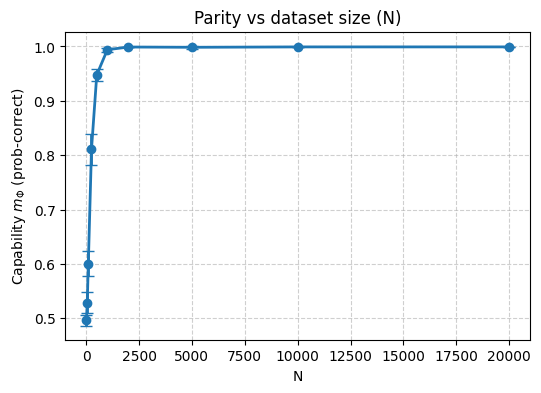
\includegraphics[width=0.65\textwidth]{A1_parity/parity_N.png}
    \caption{Capability $m_\Phi$ vs.~training tokens $T$. Error bars represent $\pm$1 std.~dev across seeds.}
    \label{fig:mphi-scaling}
\end{figure}

\begin{table}[h]
\centering
\begin{tabular}{rccc}
\toprule
$N$ (training size) & $m_\Phi$ & $\pm$ std.~dev. & Notes \\
\midrule
10  & 0.4959655 & 0.009785 & abccc \\
50  & 0.528840 &  0.020138 & abccc \\
100 & 0.600190 & 0.022990 & abccc \\
250 & 0.810683 & 0.028369 & abccc \\
500 & 0.947869 & 0.011377 & abccc \\
1000 & 0.994044 & 0.003330 & abccc \\
2000 & 0.998997 & 0.000836 & abccc \\
5000 & 0.998513 & 0.002875 & abccc \\
10000 & 0.999188 & 0.000308 & abccc \\
20000 & 0.999216 & 0.000561 & abccc \\

\bottomrule
\end{tabular}
\caption{Seed-averaged capability scores $m_\Phi$ as a function of training size $N$.}
\label{tab:mphi-results}
\end{table}
\clearpage

\begin{figure}[h]
    \centering
    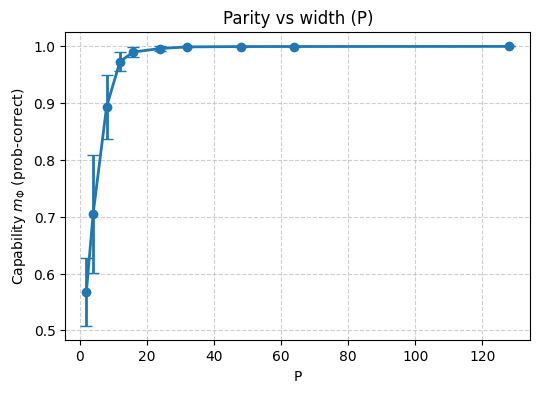
\includegraphics[width=0.65\textwidth]{A1_parity/parity_P.png}
    \caption{Capability $m_\Phi$ vs.~hidden width $P$. Error bars represent $\pm$1 std.~dev across seeds.}
    \label{fig:mphi-scaling}
\end{figure}

\begin{table}[h]
\centering
\begin{tabular}{rccc}
\toprule
$N$ (training size) & $m_\Phi$ & $\pm$ std.~dev. & Notes \\
\midrule
2  & 0.568036 & 0.059987 & abccc \\
4  & 0.704992 &  0.103550 & abccc \\
8 & 0.893279 & 0.056577 & abccc \\
12 & 0.973216 & 0.016356 & abccc \\
16 & 0.989956 & 0.009209 & abccc \\
24 & 0.996192 & 0.004893 & abccc \\
32 & 0.998997 & 0.000836 & abccc \\
48 & 0.999625 & 0.000100 & abccc \\
64 & 0.999681 & 0.000316 & abccc \\
128 & 0.999885 & 0.000025 & abccc \\
\bottomrule
\end{tabular}
\caption{Seed-averaged capability scores $m_\Phi$ as a function of training size $N$.}
\label{tab:mphi-results}
\end{table}
\clearpage

\begin{figure}[h]
    \centering
    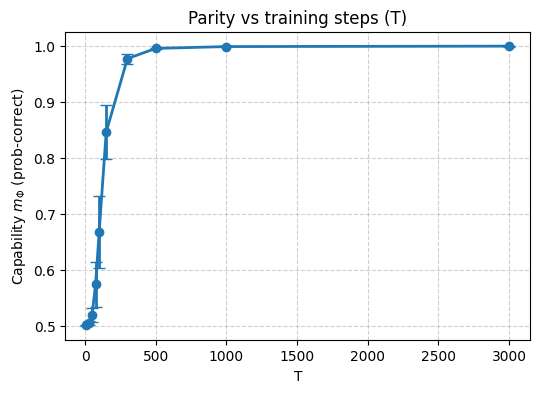
\includegraphics[width=0.65\textwidth]{A1_parity/parity_T.png}
    \caption{Capability $m_\Phi$ vs.~training steps $T$. Error bars represent $\pm$1 std.~dev across seeds.}
    \label{fig:mphi-scaling}
\end{figure}

\begin{table}[h]
\centering
\begin{tabular}{rccc}
\toprule
$N$ (training size) & $m_\Phi$ & $\pm$ std.~dev. & Notes \\
\midrule
10  & 0.501841 & 0.000950 & abccc \\
30  & 0.506235 &  0.003317 & abccc \\
50 & 0.520094 & 0.011847 & abccc \\
75 & 0.574808 & 0.040671 & abccc \\
100 & 0.667526 & 0.064508 & abccc \\
150 & 0.846540 & 0.047339 & abccc \\
300 & 0.977447 & 0.008803 & abccc \\
500 & 0.995723 & 0.001264 & abccc \\
1000 & 0.998997 & 0.000836 & abccc \\
3000 & 0.999773 & 0.000736 & abccc \\

\bottomrule
\end{tabular}
\caption{Seed-averaged capability scores $m_\Phi$ as a function of training size $N$.}
\label{tab:mphi-results}
\end{table}
\clearpage

In this first experiment, I attempted to test Axiom 1 (monotonicity of capability with respect to resources) on the parity capability using multilayer perceptrons (MLPs). I systematically varied all three resource coordinates: the number of training examples $N$, hidden width $P$, and training steps $T$. I also explored different depths, activation functions, learning rates, and data sizes. Across all settings, the seed-averaged capability score $m_\Phi$ remained flat at chance level ($ \approx 0.5$) with only random noise fluctuations, regardless of how resources were scaled. Consequently, the resulting plots were effectively random up-and-down wiggles with no interpretable monotonic trend.

This shows that for parity at input length $L=32$, the MLP family $F$ I tested is unable to represent the capability at all: increasing resources does not move performance above chance. What initially looked like a falsification of Axiom 1 is better interpreted as a gap in the axiom’s formulation. Monotonicity should not be assumed universally; it only makes sense once the capability is within the representational reach of the system $S$. In other words, Axiom 1 requires a precondition: if a system cannot express a capability, scaling resources does not guarantee improvement. This is what I talk more about in the next experiment.

The parity experiment thus provides my first concrete evidence that monotonicity axioms must be conditional on representability. While the immediate plots are uninformative, the exercise clarified a critical theoretical direction: embedding representability into the axioms themselves so that empirical results align naturally with the formal framework.

\clearpage

\subsection{Validity of Representability}

This is the experiment I did to arrive at a definition of representability.

\clearpage

\subsection{A5: Testing local continuity between recipes and the learning system}

\subsubsection{Overview}

In this experiment we fix data $D$ and resources $R$, and we jitter the recipe $\Xi$ (learning rate, width, seed, etc), giving us multiple recipes $\Xi_1,\Xi_2,\dots$, and in turn multiple learning systems $\Xi_1\times D, \Xi_2\times D,\dots$. We then train each learning system once (sampling a $\theta$ from the training kernel), and compare the induced precitor maps $\Pi_\theta$ via their capacity score $M_\Phi(\theta)$.

By axiom 5, it should be the case that varying the recipe slightly within its neighborhood in $(\mathcal R, \tau_\mathcal R)$, the emergent capability function (parity), $m_\Phi((D,\Xi),R)$ varies continuously with respect to those perturbations. This is what we are testing. 

So we empirically want to "prove" the continuity of the deterministic trained predictor map
\[
G:(\Xi, \omega)\mapsto \Pi_{\theta(\Xi, \omega)} \in \mathcal S _{\text{pred}}
\]
where $\omega$ is the randomness/seed. In other words, we check whether small recipe changes implies small changes in the predictor, for single seeds.

\clearpage
\subsubsection{Findings}

\begin{figure}[h]
    \centering
    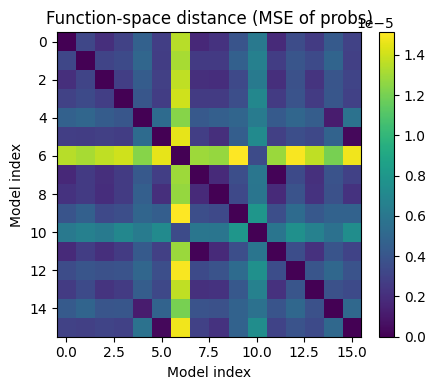
\includegraphics[width=0.65\textwidth]{figures/A5/local continuity/function-space distance.png}
\end{figure}

\begin{figure}[h]
    \centering
    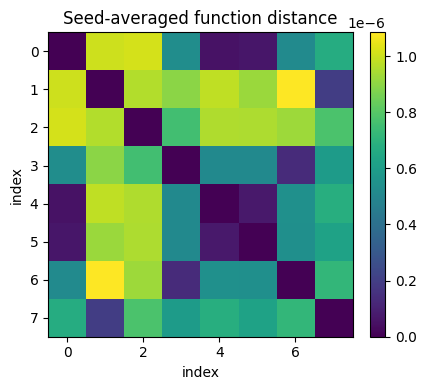
\includegraphics[width=0.65\textwidth]{figures/A5/local continuity/m_phi function distance.png}
\end{figure}

\begin{figure}[h]
    \centering
    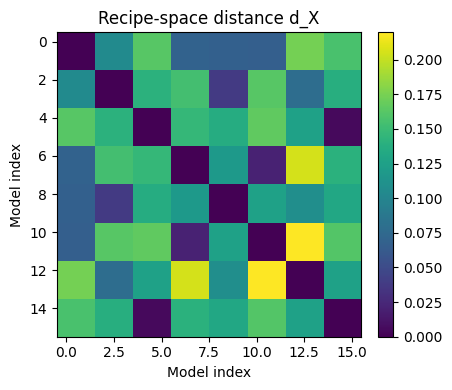
\includegraphics[width=0.65\textwidth]{figures/A5/local continuity/recipe-space distance.png}
\end{figure}

\begin{figure}[h]
    \centering
    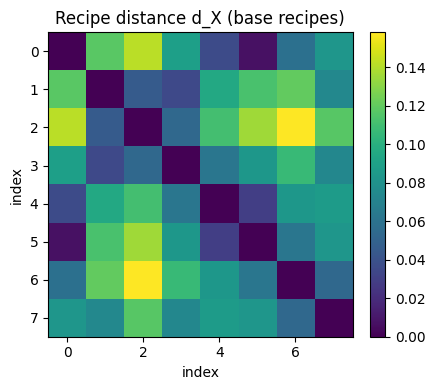
\includegraphics[width=0.65\textwidth]{figures/A5/local continuity/recipe distance base recipes.png}
\end{figure}

\begin{figure}[h]
    \centering
    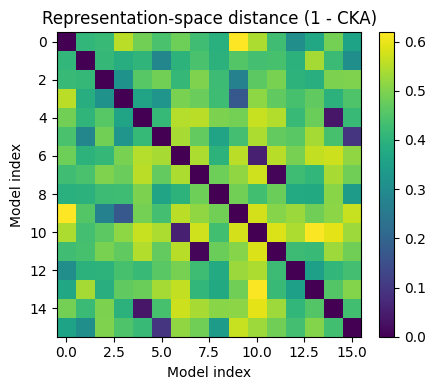
\includegraphics[width=0.65\textwidth]{figures/A5/local continuity/representation-space distance.png}
\end{figure}

\begin{figure}[h]
    \centering
    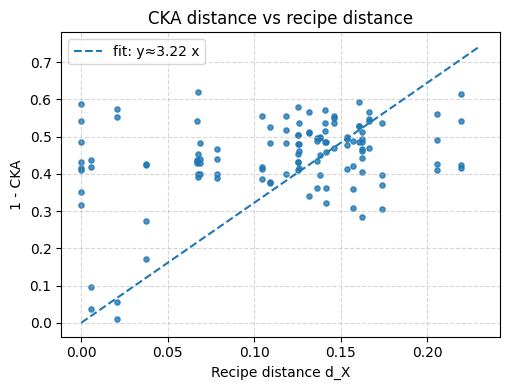
\includegraphics[width=0.65\textwidth]{figures/A5/local continuity/cka distance vs recipe distance.png}
\end{figure}

\begin{figure}[h]
    \centering
    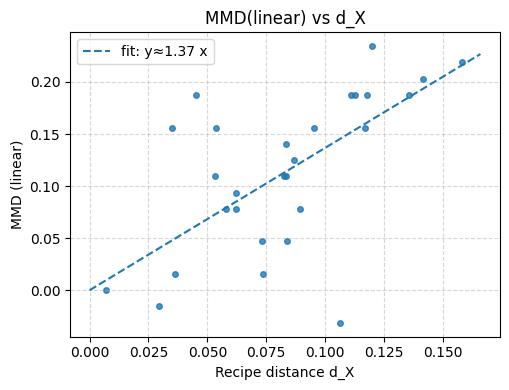
\includegraphics[width=0.65\textwidth]{figures/A5/local continuity/linear kernel vs function distance.png}
\end{figure}

\begin{figure}[h]
    \centering
    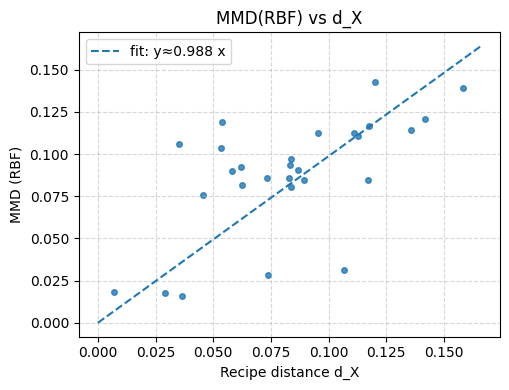
\includegraphics[width=0.65\textwidth]{figures/A5/local continuity/rbf kernel vs function distance.png}
\end{figure}

\begin{figure}[h]
    \centering
    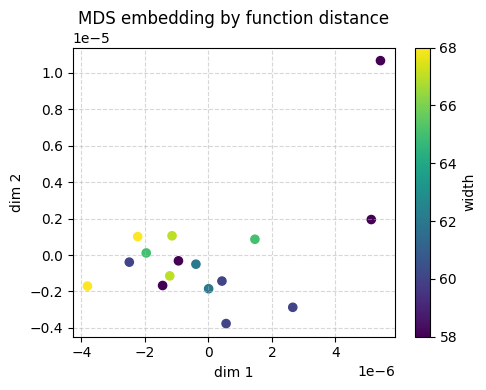
\includegraphics[width=0.65\textwidth]{figures/A5/local continuity/mds embedding by function distance.png}
\end{figure}

\begin{figure}[h]
    \centering
    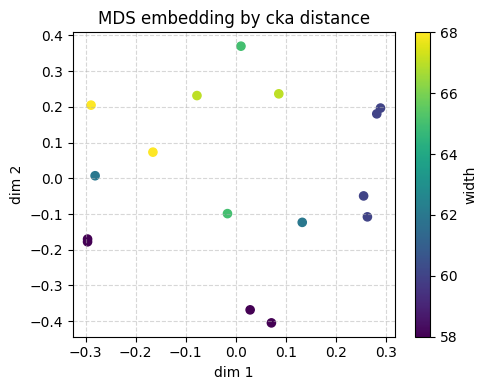
\includegraphics[width=0.65\textwidth]{figures/A5/local continuity/mds embedding by cka distance.png}
\end{figure}

I also did an openness test for $R_\tau$ where $\tau = 0.90$:
\begin{itemize}
    \item $|R_\tau|$ (by lower CI): 8/8
    \item openness radius (median / mean $\pm$ sd): $0.1278 / 0.1309 \pm  0.0191$
\end{itemize}

Seed-avg Lipschitz $L$ (func): $7.44e-06$, $R^2=0.472$

\begin{figure}[h]
    \centering
    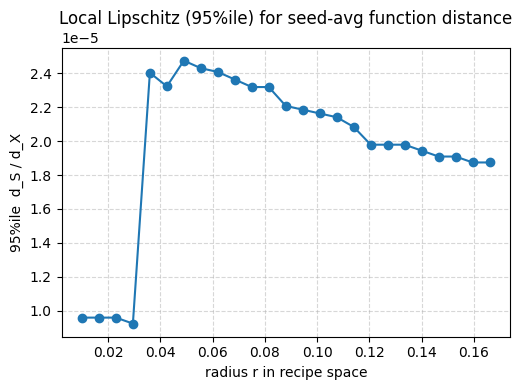
\includegraphics[width=0.65\textwidth]{A5/local continuity/local lipshitz for m_phi function distance.png}
\end{figure}

\clearpage
\subsubsection{Conclusions}

Thus, we've gathered concrete evidence that in function space the predictor varies continuously and very weakly under local recipe perturbations. So this experiment justifies the "nearby recipes leads to nearby systems" intuition. Note that this is a local continuity result for $G$, not yet for $K$, the training map.

Axiom 5 is an assumption of structure, and not a continuity claim by itself. To motivate it further we want to show that reasonable metrics/topologies on $\mathcal S$ lead to reasonable neighborhoods in $\mathcal S$. Tiny jitters in some $\Xi$ or $D$ shouldn't cause wild, discontinuous jumps in the trained learning system's behavior.

The current results already supports this specifically \textit{for outputs}: 
\[
\text{tiny } d_X\Longrightarrow d_\text{func} \approx 10^{-5}
\]

That is, nearby recipes induce almost identical predictions. 95-percentage distances inside small $d_X$ balls are $\sim 10^{-5}$. Conclusively, the experiment supports using the proposed $d_X$ to topologize $\mathcal R$ and support local continuity of the recipe-to-system map in outputs. 

\subsubsection{Representation-space continuity}

During the same experiment, we don't have reasonable evidence to conclude anything about the representation space. It is inconclusive for representation geometry and does not yet test the stochastic training kernel continuity. The $1-\text{CKA}$ is much larger, with median $\sim 0.5-0.6$, and highly variable even under the tiny recipe changed made. So nearby recipes might yield representionally different learning systems. 

Secondly, simple linear fits give tiny positive slopes but negative $R^2$ for both spaces. There’s some monotone relationship with recipe distance, but high variance means we cannot draw a quantitative law yet.

Lightbulb!!! Right now Axiom 5 is very general, and while it is hard to justify in it of itself, this experiment might suggest that this axion is empirically well-motivated only at the level of predictor outputs. For representations, continuity is not guaranteed.

% right before \appendix
\clearpage
\appendix

\section{Historical Axioms}
% Local (section-scoped) contents to navigate axiom histories:
\etocsettocstyle{\subsection*{Historical Axioms — Contents}}{} % heading for the local ToC
\localtableofcontents
\medskip

% --- Axiom 1 history ---
\subsection{Axiom 1: Monotone Capability}

\begin{histaxiom}[v0.0 — 2025-08-23]
\textbf{Status:} Retired.

\textbf{Old statement.}
Fix a learning system $S$ (as defined in the domain) and a capability $\Phi$. The order parameter $m_\Phi(S,R)\in[0,1]$ is **non-decreasing** in each resource coordinate of $R$
when the others are held fixed:

\[
\nabla _{ R} m_\Phi (S,R)\ge 0,
\]

with derivatives interpreted in a discrete sense when resources change in steps.

\textbf{Issue.}
The axiom failed if the capability/task wasn't \textit{representable} by the learning system. As shown in experiments, for example, a 4-layer MLP can't perform well on a parity task with input lengths of 32. Thus, it is stuck at random guessing which didn't change no matter how much the resources in was increased. 

The axiom also failed due to numerical fluctuations.

\textbf{Solution.}
TBD.

\end{histaxiom}



% --- Axiom 2 history ---
\subsection{Axiom 2: One-Dimensional Collapse}

\begin{histaxiom}[Axiom 2 — v0.2 — 2025-07-22]

\end{histaxiom}

\subsection{Axiom 5: Topology}

\begin{histaxiom}[Axiom 5 - v0.0 - 2025-09-03]
\textbf{Status:} Retired.
\textbf{Old statement.}
The collection of data-generating processes forms a topological space $(\mathcal D, \tau_D)$ and the collection of recipes forms a topological space $(\mathcal R, \tau_\mathcal R)$.

\textbf{Issue And Solution.}
We don’t have reasonable evidence to conclude anything about
the representation space. It is inconclusive for representation geometry and does not yet
test the stochastic training kernel continuity. 

The theory might be more useful when speaking strictly about behavioral continuity under scaling, not about representational continuity. Thus, we add a precondition to axiom 5.
    
\end{histaxiom}


\end{document}
